\documentclass{training}
\usepackage{lscape}

\title{KiCad training}
\date{\today}
\author{Blaise Thompson}

\begin{document}

\maketitle
\renewcommand{\baselinestretch}{0.5}\normalsize
\tableofcontents
\renewcommand{\baselinestretch}{1.0}\normalsize
\vfill

Part of the training materials prepared by the \href{https://shops.chem.wisc.edu/}{Chemistry Shops} at UW--Madison. \\
Source code and all associated files can be found at \href{https://github.com/uw-madison-chem-shops/training}{GitHub}. \\
If you find any mistakes or feel that any information is missing, please \href{https://github.com/uw-madison-chem-shops/training/issues}{open an issue}. \\

\clearpage

\begin{landscape}
\begin{tabular}{l | l | l}
    reference  & symbol & footprint \\ \hline
    C1         & Device:C\_Polarized\_US & Capacitor\_THT:CP\_Radial\_D7.5mm\_P2.50mm \\
    C2         & Device:C\_Polarized\_US & Capacitor\_THT:CP\_Radial\_D7.5mm\_P2.50mm \\
    C3         & Device:C\_Polarized\_US & Capacitor\_THT:CP\_Radial\_D7.5mm\_P2.50mm \\
    C4         & Device:C & Capacitor\_THT:CP\_Radial\_D7.5mm\_P2.50mm \\
    C4         & Device:C & Capacitor\_THT:CP\_Radial\_D7.5mm\_P2.50mm \\
    J\_INPUT   & Connector\_Generic:Conn\_01x02 & Connector\_Molex:Molex\_KK-254\_AE-6410-02A\_1x02\_P2.54mm\_Vertical \\
    J\_OUTPUT  & Connector\_Generic:Conn\_01x02 & Connector\_Molex:Molex\_KK-254\_AE-6410-02A\_1x02\_P2.54mm\_Vertical \\
    J\_POWER   & Connector\_Generic:Conn\_01x02 & Connector\_Molex:Molex\_KK-254\_AE-6410-02A\_1x02\_P2.54mm\_Vertical \\
    R1         & Device:R\_US & Resistor\_THT:R\_Axial\_DIN0207\_L6.3mm\_D2.5mm\_P7.62mm\_Horizontal \\
    R2         & Device:R\_US & Resistor\_THT:R\_Axial\_DIN0207\_L6.3mm\_D2.5mm\_P7.62mm\_Horizontal \\
    R\_DELAY   & Device:R\_Variable\_US & Connector\_Molex:Molex\_KK-254\_AE-6410-02A\_1x02\_P2.54mm\_Vertical \\
    R\_GATE    & Device:R\_Variable\_US & Connector\_Molex:Molex\_KK-254\_AE-6410-02A\_1x02\_P2.54mm\_Vertical \\
    TP\_5V     & Connector:TestPoint & TestPoint:TestPoint\_Loop\_D2.60mm\_Drill1.6mm\_Beaded \\
    TP\_COM    & Connector:TestPoint & TestPoint:TestPoint\_Loop\_D2.60mm\_Drill1.6mm\_Beaded \\
    TP\_DELAY  & Connector:TestPoint & TestPoint:TestPoint\_Loop\_D2.60mm\_Drill1.6mm\_Beaded \\
    TP\_INPUT  & Connector:TestPoint & TestPoint:TestPoint\_Loop\_D2.60mm\_Drill1.6mm\_Beaded \\
    TP\_OUTPUT & Connector:TestPoint & TestPoint:TestPoint\_Loop\_D2.60mm\_Drill1.6mm\_Beaded \\
    U1         & Regulator\_Linear:L7805 & Package\_TO\_SOT\_THT:TO-220-3\_Vertical \\
    U2         & 74xx:74LS121 & Package\_DIP:DIP-16\_W7.62mm\_LongPads \\
    U3         & 74xx:74LS121 & Package\_DIP:DIP-16\_W7.62mm\_LongPads \\
    mounting   & & MountingHole\_3.2mm\_M3
\end{tabular}
\end{landscape}


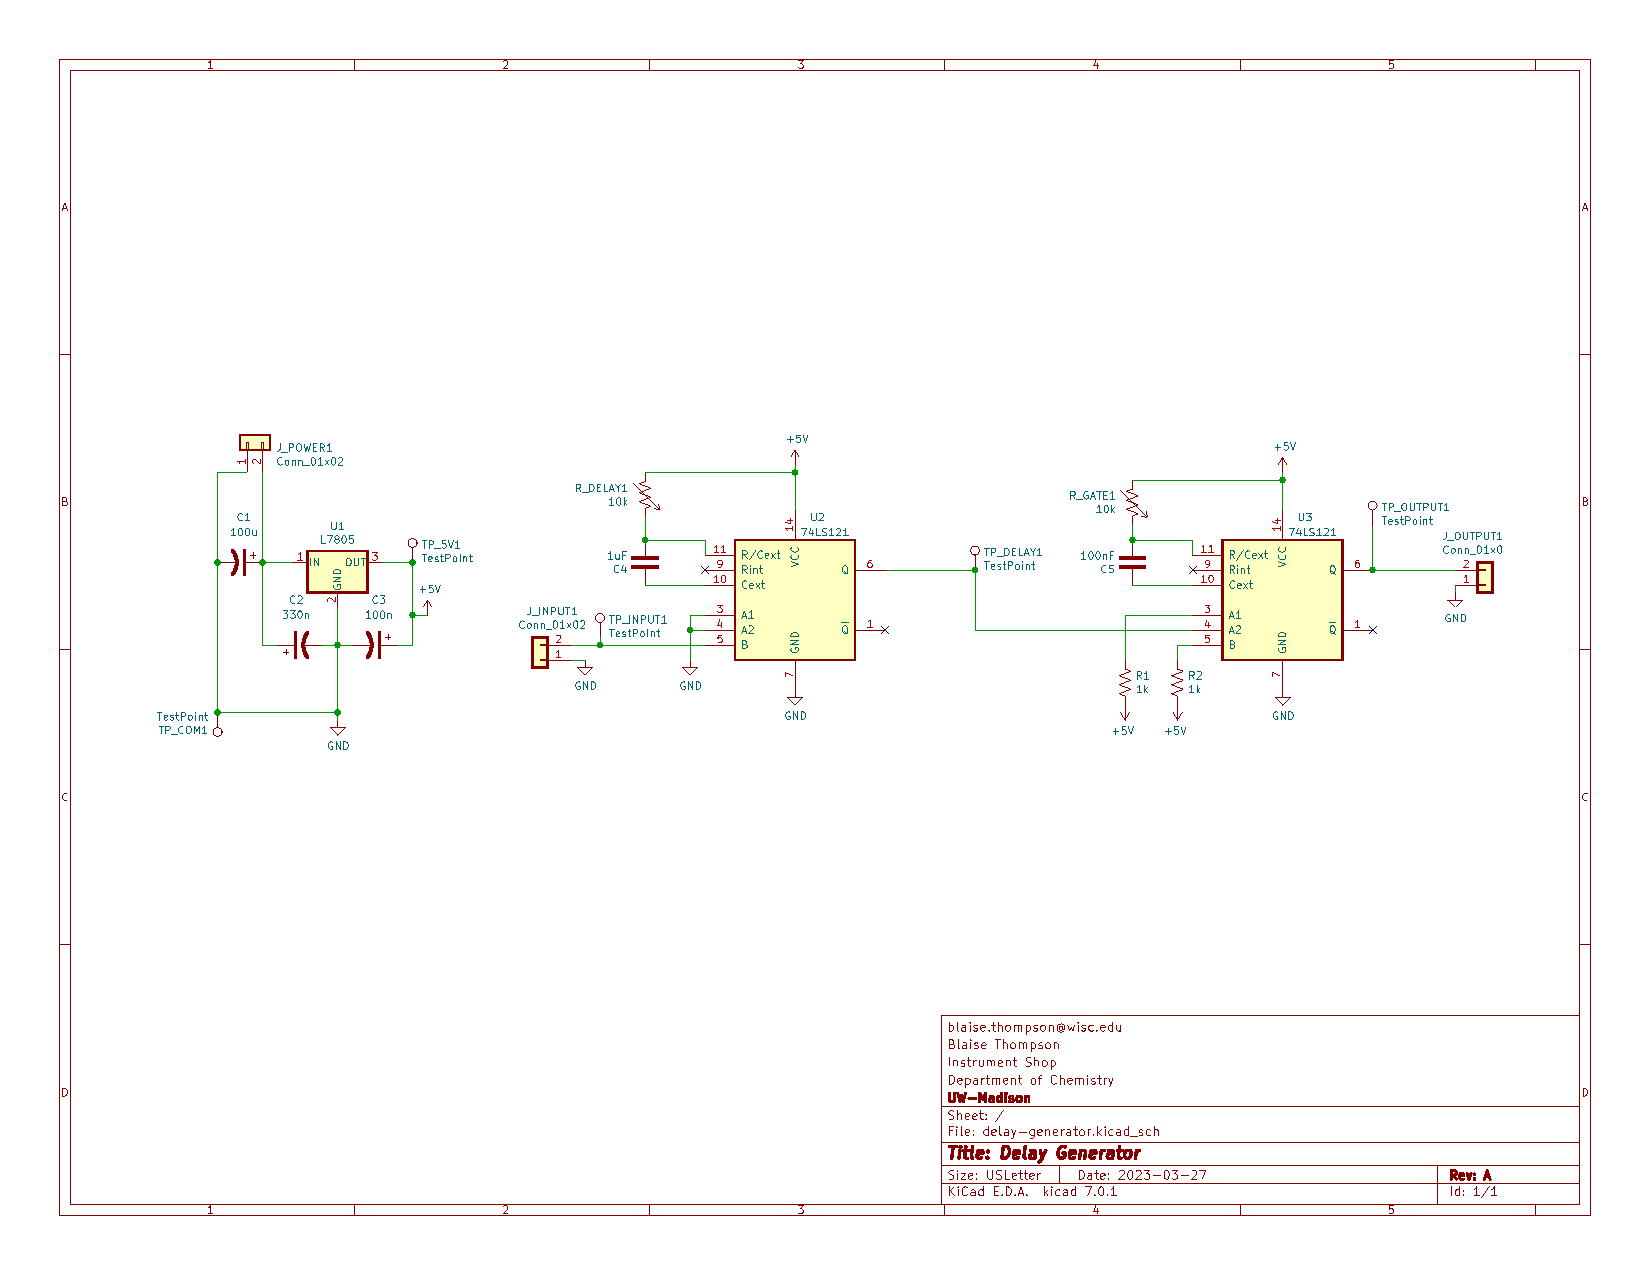
\includepdf[pages=-, landscape]{"../delay-generator.pdf"}
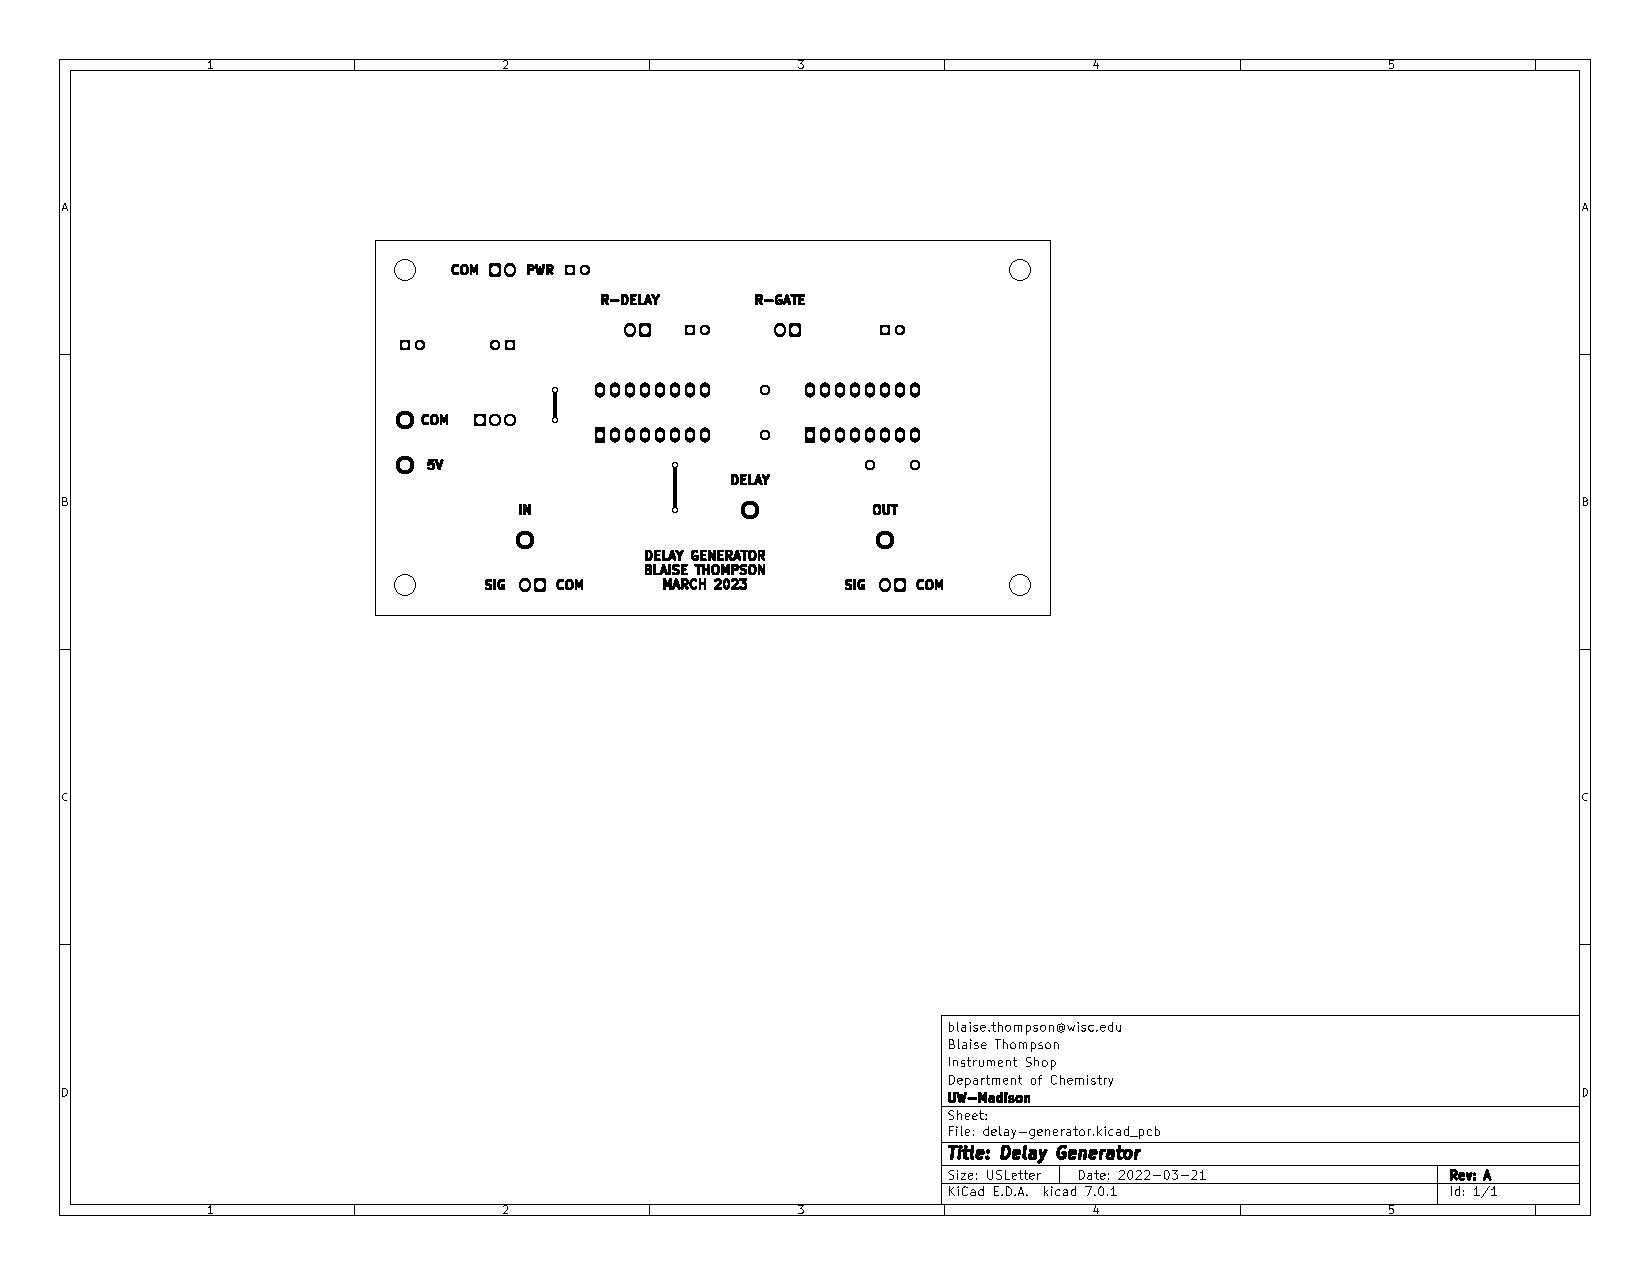
\includepdf[pages=-, landscape]{"../delay-generator-F_Cu.pdf"}
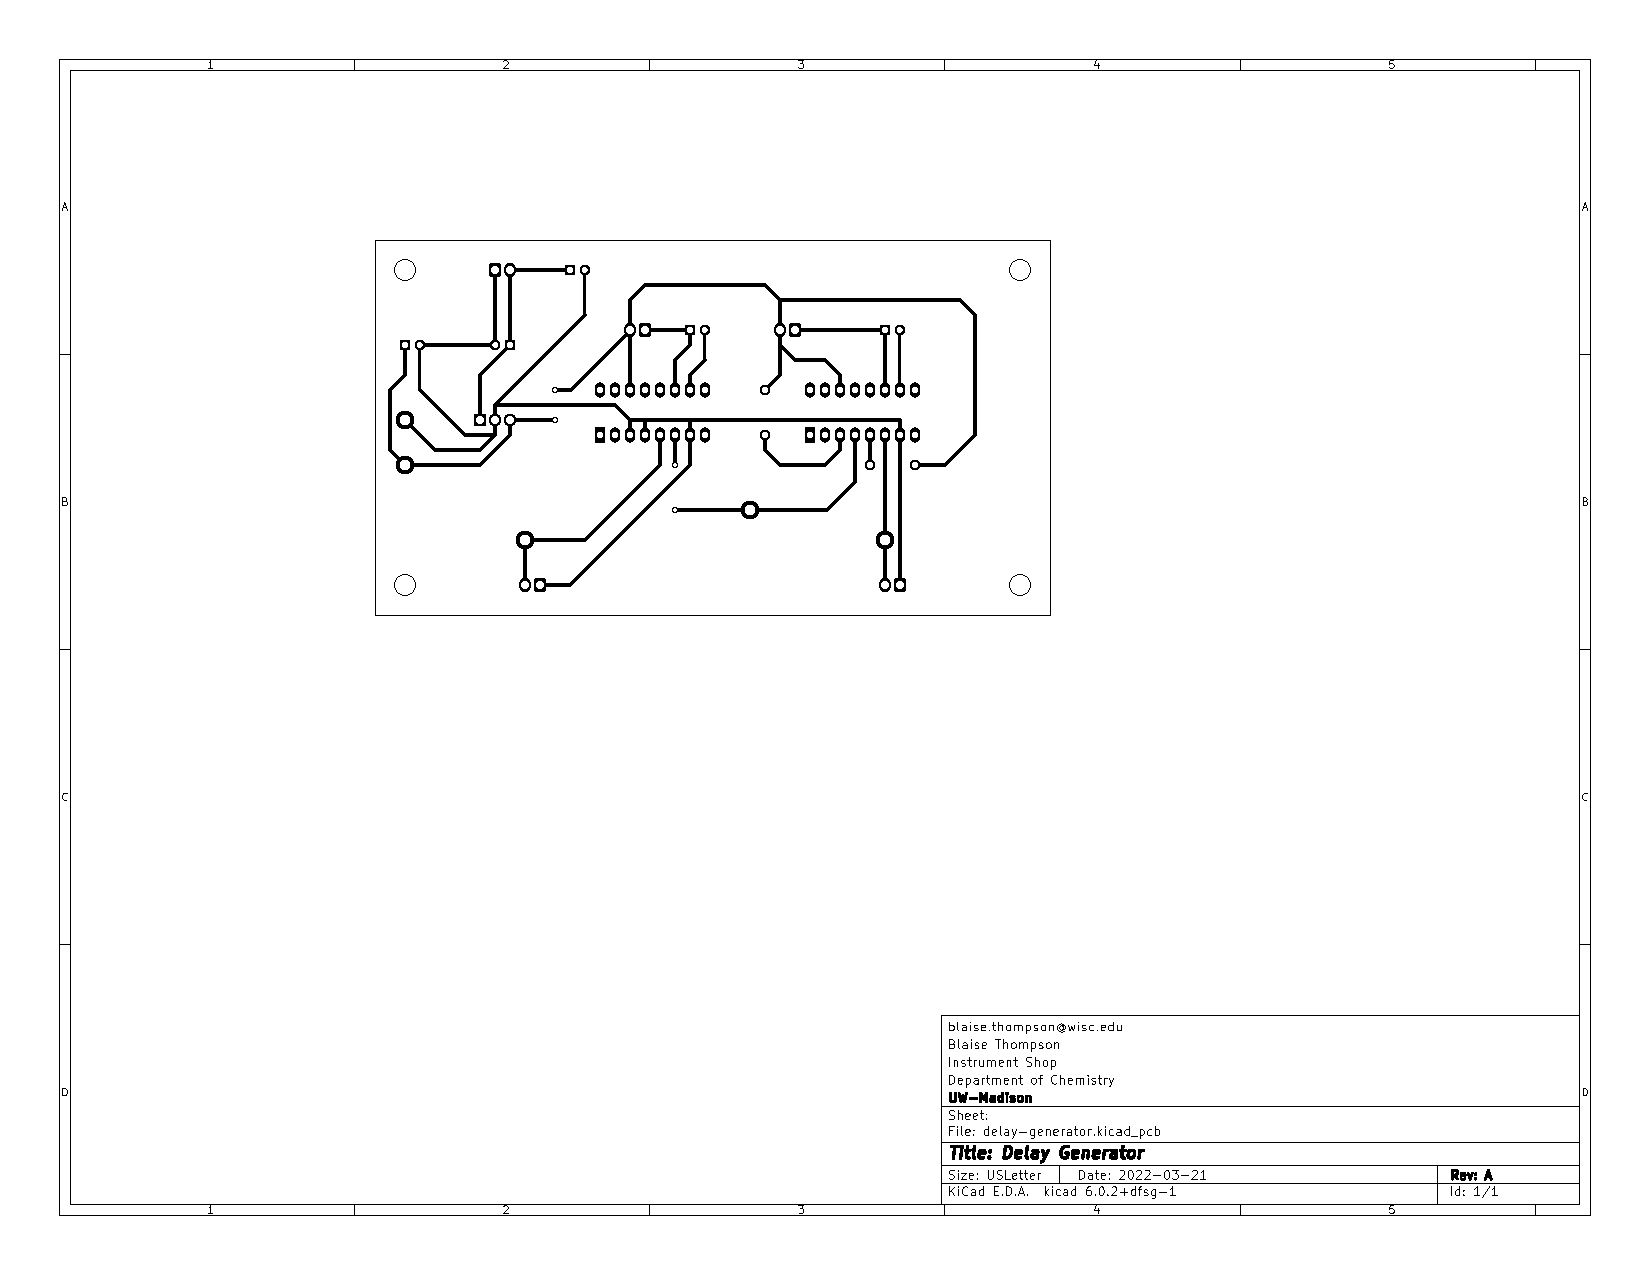
\includepdf[pages=-, landscape]{"../delay-generator-B_Cu.pdf"}




\clearpage
\section{electronic computer-aided design}

Various options, including:
\begin{itemize}
  \item EAGLE (part of autodesk family)
  \item ExpressPCB
  \item KiCAD
  \item Altium
  \item Cadence OrCAD
\end{itemize}
Prefer KiCad.

Most ECAD programs have two main interfaces to the circuit:
\begin{enumerate}
  \item The schematic
  \item The PCB
\end{enumerate}

\clearpage
\section{introduction to KiCad}

download from http://kicad-pcb.org/download/

When you first launch KiCad, you will be met with a totally blank application.

KiCad is actually made up of several sub-programs.
You will see these listed along the top of the page.
They include:
\begin{itemize}
  \item schematic layout editor
  \item symbol library editor
  \item PCB layout editor
  \item footprint library editor
  \item gerber viewer
  \item import bitmap
  \item calculator
  \item worksheet layout editor
\end{itemize}

For this introduction, we will be building a simple delay generator circuit from 628.

\subsection{creating a project}

Before we create our first project, a word about staying organized.
A KiCad project is not a single file.
Instead, a KiCad project is a \emph{folder} with different files corresponding to different pieces of your project, like the schematic and (when appropriate) PCB.
Furthermore, you will find yourself using and modifying \emph{libraries} of electronic footprints and symbols---these will also become part of your project.
It is imperative that the contents of this folder remain organized, or you risk ``breaking'' your project.

Use File New Project to create a new project.
Choose the location and name of your new project.
You will find that KiCad creates a folder at your chosen location.
That folder is immediately populated with three files:
\begin{itemize}
  \item kicad\_pcb
  \item pro
  \item sch
\end{itemize}


\clearpage
\section{schematic capture using eeschema}


Change page layout.

\clearpage
\section{pcb layout using pcbnew}

Change page layout.



\end{document}
